\section{Yarn}

An acronym for "Yet Another Resource Negotiator", Yarns responsibility is scheduling of jobs on the cluster and was added in version 2.x of Hadoop \cite[pg.1]{yarn-scheduling}.

Yarn is made up of 2 components, the Resource Manager and the Node Manager. The resource manager runs on the master node, while the node manager runs on every node in the cluster. The responsibility of the resource manager is to monitor all resources across the cluster, such as cpu and memory. The node manager is only concerned with monitoring the resources on its current node.

Yarn has a number of of different scehduling options we can choose from. Some options are \cite[pg.2]{yarn-scheduling}

\begin{itemize}
\item First In First Out Scheduler 
\item Capacity Scheduler
\item Fair Scheduler 
\item Dominant Resource Fairness
\item Label Based Scheduling
\item HaSTE
\end{itemize}

For the purposes of this paper we will outline the first 3 types of scheduling in .

\subsection{First In First Out Scheduler}

This schedular is similar to a queue. A good analygy might be that we are waiting in a queue at the bank with only one teller. If we are the third person in the queue we will have to wait for person 1 and then person 2 to complete their transactions before we have access to the teller. 
There is one major drawback to this approach. One single job no matter how big or small will take up all the resources on the cluster even if some resources are not used. This can result in long waiting times for jobs to complete.

\begin{figure}[H]
  \centering
  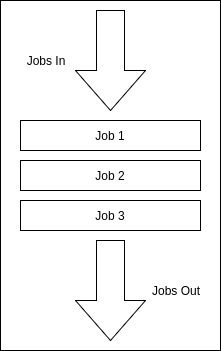
\includegraphics[scale=0.7]{./images/fifo-scheduler.png}
  \caption{FIFO queue}
  \label{fig:fifo-scheduler}
\end{figure}

\subsection{Capacity Scheduler}